\documentclass[12pt]{article}
\usepackage[utf8]{inputenc}
\usepackage[spanish]{babel}
\usepackage{amsmath,amssymb}
\usepackage{booktabs}
\usepackage{xcolor}
\usepackage{graphicx}
\usepackage{geometry}
\geometry{margin=2.5cm}
\usepackage{fancyhdr}
\pagestyle{fancy}
\fancyhf{}
\rhead{Investigación de Operaciones}
\lhead{Método Simplex}

\title{Resultados del Método Simplex\\
\large Problema: \textbf{1}}
\author{
Emily Sánchez\\
Viviana Vargas\\
\\
Curso: Investigación de Operaciones\\
Semestre: 2024-1
}
\date{\today}

\begin{document}

\maketitle
\thispagestyle{empty}

\vfill
\begin{center}
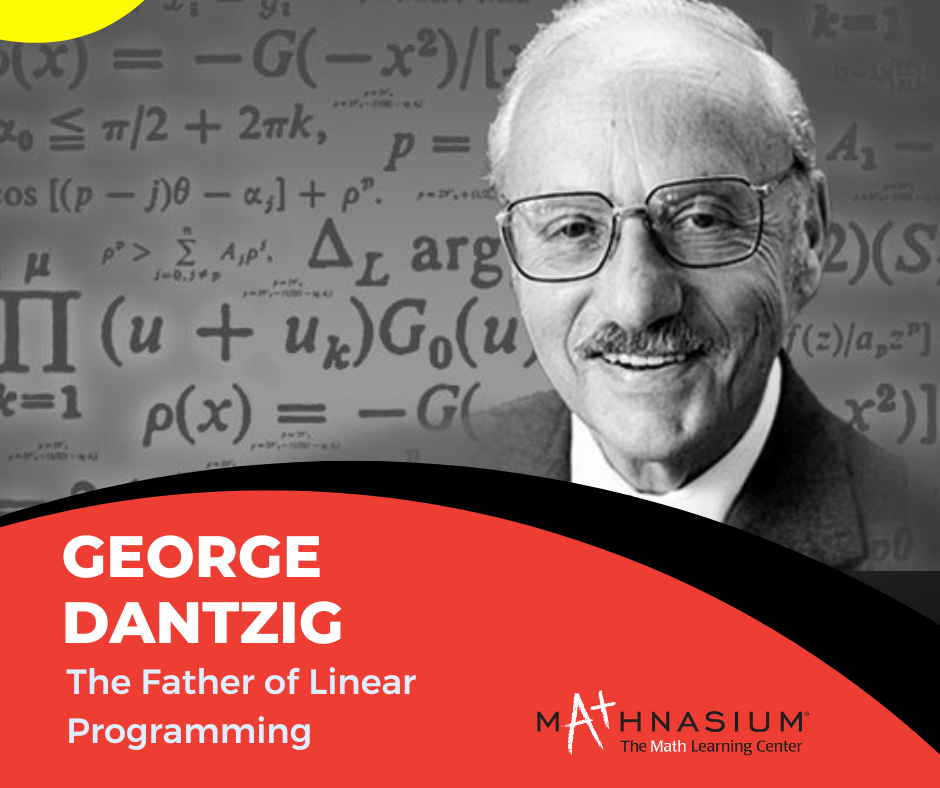
\includegraphics[width=0.3\textwidth]{dantzig}
\\
\small George Dantzig (1914-2005)
\\
Creador del Método Simplex
\end{center}
\vfill

\newpage
\tableofcontents
\newpage
\section{El Algoritmo Simplex}

\subsection{Historia}
El método Simplex fue desarrollado por George Dantzig en 1947 mientras trabajaba para la Fuerza Aérea de los Estados Unidos. \\

Es uno de los algoritmos más importantes en la historia de la optimización matemática y ha sido fundamental en el desarrollo de la programación lineal.

\subsection{Propiedades Fundamentales}
\begin{itemize}
\item \textbf{Convergencia:} El algoritmo converge a la solución óptima en un número finito de pasos (en la mayoría de los casos prácticos)
\item \textbf{Complejidad:} En el peor caso tiene complejidad exponencial, pero en la práctica es muy eficiente
\item \textbf{Optimalidad:} Garantiza encontrar la solución óptima global para problemas convexos
\item \textbf{Factibilidad:} Mantiene la factibilidad en cada iteración
\end{itemize}

\subsection{Descripción del Método}
El método Simplex opera moviéndose entre vértices adyacentes del poliedro factible, mejorando el valor de la función objetivo en cada paso hasta alcanzar el óptimo.

\section{Problema Original}

\subsection{Formulación Matemática}
\textbf{Problema de Maximización}

\[ \text{Maximizar } Z = 3X1 + 4X2 \]

\textbf{Sujeto a:}
\begin{align*}
1X1 + 1X2 &\leq 40 \\
1X1 + 2X2 &\leq 60
\end{align*}

\textbf{Con:}
\[ X1 \geq 0, \quad X2 \geq 0 \]

\section{Tabla Inicial}

La tabla inicial del método Simplex incluye las variables de holgura para convertir las desigualdades en igualdades.

\begin{center}
\small
\begin{tabular}{|c|c|c|c|c|c|}
\hline
 & \textbf{X1} & \textbf{X2} & \textbf{$s_1$} & \textbf{$s_2$} & \textbf{L.D.} \\
\hline
\textbf{Z} & 3 & 4 & 0 & 0 & 0 \\
\hline
\textbf{$s_1$} & 1 & 1 & 1 & 0 & 40 \\
\hline
\textbf{$s_2$} & 1 & 2 & 0 & 1 & 60 \\
\hline
\end{tabular}
\end{center}

\section{Tablas Intermedias}

A continuación se presentan las tablas intermedias generadas durante la ejecución del algoritmo Simplex.

\subsection{Iteración 0}
\begin{center}
\small
\begin{tabular}{|c|c|c|c|c|c|}
\hline
 & \textbf{X1} & \textbf{X2} & \textbf{$s_1$} & \textbf{$s_2$} & \textbf{L.D.} \\
\hline
\textbf{Z} & 3 & 4 & 0 & 0 & 0 \\
\hline
\textbf{$s_1$} & 1 & 1 & 1 & 0 & 40 \\
\hline
\textbf{$s_2$} & 1 & 2 & 0 & 1 & 60 \\
\hline
\end{tabular}
\end{center}

\subsection{Iteración 1}
\begin{center}
\small
\begin{tabular}{|c|c|c|c|c|c|}
\hline
 & \textbf{X1} & \textbf{X2} & \textbf{$s_1$} & \textbf{$s_2$} & \textbf{L.D.} \\
\hline
\textbf{Z} & 1 & 0 & 0 & -2 & -120 \\
\hline
\textbf{$s_1$} & 0.50 & 0 & 1 & -0.50 & 10 \\
\hline
\textbf{$s_2$} & 0.50 & 1 & 0 & 0.50 & 30 \\
\hline
\end{tabular}
\end{center}

\subsection{Iteración 2}
\begin{center}
\small
\begin{tabular}{|c|c|c|c|c|c|}
\hline
 & \textbf{X1} & \textbf{X2} & \textbf{$s_1$} & \textbf{$s_2$} & \textbf{L.D.} \\
\hline
\textbf{Z} & 0 & 0 & -2 & -1 & -140 \\
\hline
\textbf{$s_1$} & 1 & 0 & 2 & -1 & 20 \\
\hline
\textbf{$s_2$} & 0 & 1 & -1 & 1 & 20 \\
\hline
\end{tabular}
\end{center}

\section{Tabla Final}

La siguiente tabla representa la solución óptima del problema:

\begin{center}
\small
\begin{tabular}{|c|c|c|c|c|c|}
\hline
 & \textbf{X1} & \textbf{X2} & \textbf{$s_1$} & \textbf{$s_2$} & \textbf{L.D.} \\
\hline
\textbf{Z} & 0 & 0 & -2 & -1 & -140 \\
\hline
\textbf{$X1$} & 1 & 0 & 2 & -1 & 20 \\
\hline
\textbf{$X2$} & 0 & 1 & -1 & 1 & 20 \\
\hline
\end{tabular}
\end{center}

\section{Solución Óptima}

\textbf{Valor óptimo: } $Z = 140$

\textbf{Solución óptima:}
\begin{align*}
X1 &= 20 \\
X2 &= 20
\end{align*}

\textbf{Tipo:} Solución Única

El problema tiene una única solución óptima en el punto encontrado.

\textbf{Iteraciones realizadas:} 2

\end{document}
